% !TeX document-id = {b5392a94-51a3-49d1-9ba5-698bc09f9d35}
% !TeX encoding = UTF-8
% !TeX spellcheck = en_US
% !TeX TXS-program:bibliography = biber -l zh__pinyin --output-safechars %

\documentclass[a4paper
	,10pt
%	,twoside
]{article}

% to be `\input` in subfolders,
% ... therefore the path should be relative to subfolders.

\usepackage{iftex}
\ifPDFTeX
\else
	\usepackage[UTF8
		,heading=false
		,scheme=plain % English Document
	]{ctex}
\fi
%\ctexset{autoindent=true}
\usepackage{indentfirst}

\input{../.modules/basics/macros.tex}
\input{../.modules/preamble_base.tex}
\input{../.modules/preamble_beamer.tex}
\input{../.modules/basics/biblatex.tex}


%Misc
	\usepackage{lilyglyphs}
	\newcommand{\indicator}{$\text{\clefG}$}
	\newcommand{\indicatorInline}{$\text{\clefGInline}$}

\newcommand{\legacyReference}{{
%	\clearpage\par
%	\quad\clearpage
	\def{\midquote}{\textbf{PAST WORK, AS TEMPLATE}}
	\newparagraph
}}

% Settings
\counterwithout{equation}{section}
\mathtoolsset{showonlyrefs=false}
%\DeclareTextFontCommand{\textbf}{\sffamily}

% Spacing
\geometry{footnotesep=2\baselineskip} % pre footnote split
\setlength{\parskip}{.5\baselineskip}
\renewcommand{\baselinestretch}{1.15}


%% List
%	\setlist*{
%		listparindent=\parindent
%		,labelindent=\parindent
%		,parsep=\parskip
%		,itemsep=1.2\parskip
%	}


\addtobeamertemplate{navigation symbols}{}{%
    \usebeamerfont{footline}%
%    \usebeamercolor[fg]{footline}%
    \hspace{1em}%
    \large\insertframenumber/\inserttotalframenumber
}

\makeatletter
\setbeamertemplate{headline}
{%
    \begin{beamercolorbox}[wd=\paperwidth,colsep=1.5pt]{upper separation line head}
    \end{beamercolorbox}
    \begin{beamercolorbox}[wd=\paperwidth,ht=2.5ex,dp=1.125ex,%
      leftskip=.3cm,rightskip=.3cm plus1fil]{title in head/foot}
      \usebeamerfont{title in head/foot}\insertshorttitle
    \end{beamercolorbox}
    \begin{beamercolorbox}[wd=\paperwidth,ht=2.5ex,dp=1.125ex,%
      leftskip=.3cm,rightskip=.3cm plus1fil]{section in head/foot}
      \usebeamerfont{section in head/foot}%
      \ifbeamer@tree@showhooks
        \setbox\beamer@tempbox=\hbox{\insertsectionhead}%
        \ifdim\wd\beamer@tempbox>1pt%
          \hskip2pt\raise1.9pt\hbox{\vrule width0.4pt height1.875ex\vrule width 5pt height0.4pt}%
          \hskip1pt%
        \fi%
      \else%  
        \hskip6pt%
      \fi%
      \insertsectionhead
    \end{beamercolorbox}
% Code for subsections removed here
}
\makeatother
\input{../.modules/basics/biblatex.tex}

\title{A Modern Take on Renormalization}
%\addbibresource{.bib}

%%% ID: sensitive, do NOT publish!
%\InputIfFileExists{../id.tex}{}{}

\usepackage{cancel}

\begin{document}
\maketitle
\pagenumbering{arabic}
\thispagestyle{empty}

\vspace*{-.5\baselineskip}
	\textbf{Reason:} The continuum limit $\Lambda\to\infty$ is \textbf{not} well-defined.
	Renormalization provides a way to \emph{define} the theory when
	$\Lambda\to\infty$.
	
	\textbf{My belief:} The only way to fully understand renormalization is
	through Wilson's arguments; all other ``interpretations'' of
	renormalization are only \emph{heuristic}.

	\textbf{Keywords:}
	\begin{itemize}[nosep,topsep=-.5\parskip]
	\item Renormalization group
	\item Counterterms
	\item Regularization and cutoff
	\end{itemize}


\setlength{\parskip}{.1\baselineskip}
\tableofcontents
\setlength{\parskip}{\parskipnorm}


\section{References}

%\noindent \textsl{Ranked by importance:}

	\begin{itemize}[parsep=0pt,itemsep=.5\parskip]
	\item David Skinner's note:
	  \begin{itemize}[nosep]
	  \item \url{https://www.damtp.cam.ac.uk/user/dbs26/AQFT.html}
	    \begin{itemize}[nosep]
	    \item \url{https://www.damtp.cam.ac.uk/user/dbs26/AQFT/Wilsonchap.pdf}
	    \item \url{https://www.damtp.cam.ac.uk/user/dbs26/AQFT/chap5.pdf}
	    \end{itemize}
	  \end{itemize}
	\item Schwartz, Chapter 15
	\item Peskin \& Schroeder, Chapter 10 \& 12
	\item Hollowood's book:
	  \begin{itemize}[nosep]
	  \item \url{https://arxiv.org/abs/0909.0859}
	  \item \url{https://link.springer.com/book/10.1007/978-3-642-36312-2}
	  \end{itemize}
	\end{itemize}

\section{Wilson's picture}
	Seed theory parameters (i.e.\ \emph{bare parameters}):
	$(Z_\phi,g,\Lambda)_0$, where $g = (m,\lambda,\cdots)$ is the collection of all possible couplings. $Z_\phi$ is the coefficient of the kinetic term.
	
	\begin{equation}
	\begin{aligned}
	  \phi_{\Lambda_0}(x)
	  \sim \int^{\Lambda_0} \dd{p}
	    e^{ip\cdot x}
	    \tilde{\phi}(p)
	  &= \int^{\Lambda} \dd{p}
	    e^{ip\cdot x}
	    \tilde{\phi}(p)
	    + \int_{\Lambda}^{\Lambda_0} \dd{p}
	    e^{ip\cdot x}
	    \tilde{\phi}(p) \\
	  &=\colon \phi_{\Lambda}(x) + \chi(x)
	\end{aligned}
	\end{equation}
	
	\begin{equation}
	\begin{aligned}
	  \DD\phi_{\Lambda_0}(x)
	  \sim \prod_{\norm{p} < \Lambda_0}
	    \dd{\tilde{\phi}(p)}
	  &= \prod_{\norm{p} < \Lambda}
	    \dd{\tilde{\phi}(p)}
	    \prod_{\Lambda < \norm{p} < \Lambda_0}
	    \dd{\tilde{\phi}(p)} \\
	  &\sim
	    \DD\phi_{\Lambda}(x)\,
	    \DD\chi(x)
	\end{aligned}
	\end{equation}
	
	\begin{equation}
	\begin{aligned}
	  \mcal{Z} (g_0,\Lambda_0)
	  &= \int \DD\phi_{\Lambda_0}
	      e^{iS[\phi_{\Lambda_0}]} \\
	  &= \int \DD\phi_{\Lambda}
	    \int \DD\chi
	      e^{iS[\phi_\Lambda + \chi]} \\
	  &=: \int \DD\phi_{\Lambda}
	      e^{iS_{\mathrm{eff}} [\phi_\Lambda]}
	  =: \mcal{Z}\pqty{g(\Lambda),\Lambda}
	\end{aligned}
	\end{equation}
	Coarse-grained parameters: $(Z_\phi,g,\Lambda)$.
	
	\textbf{Subtlety:} the notation above is only schematic; in practice we
	first Wick-rotate to Euclidean signature, so that the momentum cutoff is
	easily imposed: $\norm{p} = \sqrt{p_0^2 + \vb{p}^2} < \Lambda$. In
	Lorentzian signature, it's hard to define a covariant cutoff since
	$p_\mu p^\mu = - p_0^2 + \vb{p}^2$. This process can be made rigorous;
	just think of the 8-shaped contour in loop integrals.
	
	\textbf{Effective action:}
	\begin{equation}
	  S_{\mathrm{eff}}[\phi]
	  = -i \ln \int \DD \chi
	      e^{iS[\phi + \chi]} \\
	\end{equation}
	$\phi = \phi_\Lambda$ is treated as constant when doing
	$\int \DD \chi$. Perturbatively, we integrate over loops with $\chi$ propagators as internal lines
	\begin{equation}
	\begin{aligned}
	  \mcal{L}[\phi + \chi]
	  &= - \frac{Z_\phi}{2}\,
	      \partial_\mu (\phi + \chi)\,
	      \partial^\mu (\phi + \chi)
	    - \frac{1}{2}\, m^2
	      (\phi + \chi)^2
	    - \frac{1}{4!}\, \lambda\,
	      (\phi + \chi)^4\\
	  &= \cdots \\
	  &= \mcal{L}[\phi]
	    + \Delta\mcal{L} [\phi,\chi]
	\end{aligned}
	\end{equation}
	
	\begin{equation}
	  S_{\mathrm{eff}}[\phi_\Lambda]
	  = S[\phi_\Lambda]
	    - i \ln \int \DD \chi
	      e^{i\,\Delta S[\phi_\Lambda + \chi]} \\
	\end{equation}
	
	If $\Lambda \lesssim \Lambda_0$, then $S_{\mathrm{eff}}$ is almost
	the same as the original $S$, with minor corrections from the
	$\int \DD\chi$ term. Note that in such regularization scheme there will be no \textit{quadratic} cross terms $\sim \phi\chi,\, \pd\phi\,\pd\chi$ in the effective action, since they have orthogonal Fourier modes. However, there will be non-vanishing \textit{quartic} cross terms $\sim \phi^2\chi^2,\, \phi^3\chi$. After we integrate out $\chi$, the $\phi^2\chi^2$ term will cause a shift in $m^2$, while the $\phi^3\chi$ will generate a new $\phi^6$ vertex (by a $\chi\chi$ contraction).
	
	Note that $\mcal{Z}$ clearly does not depend on the intermediate scale $\Lambda$, and we have:
	\begin{equation}
	  0
	  = \Lambda \dv{}{\Lambda}\,
	    \mcal{Z}\pqty{g(\Lambda),\Lambda}
	  = \pqty{
	      \Lambda \pdv{}{\Lambda}
	      + \Lambda \pdv{g^{(i)}}{\Lambda}
	        \pdv{}{g^{(i)}}
	    }\,
	    \mcal{Z}\pqty{g(\Lambda),\Lambda}
	\end{equation}
	This is an example of a \textbf{RG Equation}.
\subsection{Free theory \& CFT}
	We first observe that a massless free theory with $
		\mcal{L}[\phi]
		\sim \int \dd[d]{x} (\pd\phi)^2
	$ is ``not renormalized'' when we integrate out high energy modes. Roughly speaking, we have:
	\begin{equation}
	\begin{aligned}
	  \mcal{Z}
	  &= \int \DD\phi_{\Lambda_0}
	      e^{iS[\phi_0]} \\
	  &= \int \DD\phi_{\Lambda}
	    \int \DD\chi
	      e^{iS[\phi + \chi]} \\
	  &\sim \int \DD\phi_{\Lambda}
	      e^{iS[\phi]}
	      \sqrt{Z_\phi^\#}
	\end{aligned}
	\label{eq:PI_free}
	\end{equation}
	Integrating over $\Lambda = s\Lambda_0 \le \abs{p} \le \Lambda_0$ produces the $Z_\phi$ factor, where $\#$ is the total number of modes in this range. One can give an explicit expression of $\#$ with some IR cutoff $L$.
	
	On the other hand, we can restore $\Lambda = s\Lambda_0$ back to $\Lambda_0$ by rescaling. This is easy to understand when we think of a lattice theory: to probe the IR behavor, we first ``coarse-grain'' by grouping points together, effectively lowering $\Lambda$; then we ``zoom out'' to see the bigger picture. Rescaling $\Lambda = s\Lambda_0$ back to $\Lambda_0$ is precisely the ``zooming-out'' process. 
	
	When taking $\Lambda\mapsto \Lambda_0 = \Lambda / s$, first note that the kinetic term $\int \dd[d]{x} (\pd\phi)^2$ is scale-invariant if we rescale $\phi$ accordingly:
	\begin{equation}
		\Lambda\mapsto \Lambda_0 = \Lambda / s,
	\quad
		x\mapsto x' = sx,
	\quad
		\phi(x) \mapsto
		\phi'(x') = s^{1 - \frac{d}{2}} \phi(x)
	\end{equation}
	The $s^{1 - \frac{d}{2}}$ factor is consistent with the mass dimension of $\phi$, and we have $S'[\phi'] = S[\phi]$ invariant under rescaling. 
	
	The path integral measure, however, is \textit{not} scale-invariant; we have to add back some Fourier modes in between to return the path integral back to $\Lambda_0$. Luckily, the additional modes happen to cancels out the $Z_\phi$ factor in \eqref{eq:PI_free}:
	\begin{equation}
		\sqrt{Z_\phi^\#} \DD\phi_{\Lambda}
		\sim \sqrt{Z_\phi^\#}
			\prod_{\norm{p} < \Lambda = s\Lambda_0}
			\dd{\tilde{\phi}(p)}
		= \prod_{\norm{p'} < \Lambda_0}
			\dd{\tilde{\phi}'(p')}
		\sim \DD\phi'_{\Lambda_0}
	\end{equation}
	Therefore the complete path integral is invariant under RG flow \& rescaling; $Z_\phi$ is also unchanged during this process. Therefore we can simply set $Z_\phi \equiv 1$ by an appropriate \textit{normalization} of $\phi$.
	
	One can see how this process might fail in a curved background: in flat space the Fourier modes are equally spaced, and rescaling $\DD\phi_{\Lambda}$ can be achived by simply adding back a total of $\#$ modes. However, in a curved background the Fourier modes are complicated (e.g.\ think of spherical harmonics) and we generally do not expect the Jacobian of $\DD\phi_{\Lambda} \mapsto \DD\phi'_{\Lambda_0}$ to cancel out the $Z_\phi$ factor precisely. This is a hint of \textit{Weyl anomaly} in curved backgrounds. For a concrete discussion with path integral, see \textit{Di Francesco et al}, 5.A. 
\pagebreak[4]
	
	Generally, $Z_\phi$ \textit{will} change after rescaling:
	\begin{equation}
		Z_\phi \sim \Lambda^{-2\gamma_\phi},
	\quad
		\gamma_\phi
		\mathbin{:=}
		-\frac{1}{2}\,\Lambda \pdv{\ln Z_\phi}{\Lambda}
	\end{equation}
	The scaling of $Z_\phi$ can be absorbed by \textit{field strength renormalization} (or ``wave function'' renormalization); i.e.\ if we \textit{demand} $\phi$ to retain the canonical normalization such that $Z_\phi \equiv 1$, then $\phi$ must scale with an \textit{anomalous dimension} $\gamma_\phi$:
	\begin{equation}
		\phi(x) 
		\ \longmapsto\ %
		\phi'(x') = s^{1 - \frac{d}{2} - \gamma_\phi} \phi(x)
	\end{equation}
	In practice we don't actually redefine the scaling of $\phi$, just simplify keep track of it using the $Z_\phi$ factor; but we should know that due to quantum corrections, the mass dimension of $\phi$ is, effectively,
	\begin{equation}
		\Delta_\phi
		= \frac{d}{2} - 1 + \gamma_\phi
	\end{equation}
	
	In summary, we've argued that the classical \& quantum theory of a massless free boson on flat space is \textit{scale-invariant}; $\gamma_\phi = 0$. In fact, this is a first example of free CFTs. 
	CFTs are the \textit{fixed points} of RG flow.
\subsection{Massive theory \& the space of theories}
	What about \textit{massive} free theories? We do know that they don't receive loop corrections, therefore ``invariant'' under coarse-graining; however, mass \textit{do} flow when we zoom out. This is very natural; as we zoom out the energy-momentum of all modes are enhanced by a factor of $s^{-1}$, and we have $m\mapsto m/s$. Therefore $m$ is a \textit{relevant} parameter as we flow towards IR; it grows and flows away from the massless free CFT. For an explicitly path integral calculation (along with $\phi^{2n}$ interactions), see \textit{Hollowood}, 2.1. 
	
	Generally, for small $g$ we can think of the theory $(g,\Lambda)$ as a \textit{deformation} away from the massless free CFT. A neat trick to stop worrying about rescaling is to re-define $g$ as dimensionless couplings:
	\begin{equation}
		g(\Lambda) = \pqty{
			g^{(2)} = \frac{m^2_{(\Lambda)}}{\Lambda^2},
			\ g^{(4)} = \lambda,
			\ g^{(6)} = \cdots
		}
	\end{equation}
	Here we use $m^2_{(\Lambda)}$ to denote the mass \textit{after} coarse-graining but \textit{before} rescaling. The mass term is then given by $
		\sim \int \dd[d]{x} m^2 \phi^2
		= \int \dd[d]{x} g^{(2)} \Lambda^2 \phi^2
	$. $g$ is thus invariant under rescaling, as the rescaling factor is absorbed by the $\Lambda$ factor. We also don't have to worry about the anomalous path integral measure, as it's captured by the $Z_\phi$ factor. 
	
	After rescaling $\Lambda \mapsto \Lambda_0$, the dimensionful mass is given by:
	\begin{equation}
		m'^2_{(\Lambda)}
		= g^{(2)}_{(\Lambda)} \Lambda_0^2
		= m^2_{(\Lambda)}
			\pqty{\frac{\Lambda_0}{\Lambda}}^2
	\end{equation}
	In general, the rescaled, dimensional coupling is simply the dimensionless coupling times some factors of the \textit{initial} cutoff $\Lambda_0$. Therefore its $\Lambda$ dependence is identical to that of the dimensionless coupling. On the other hand, the coarse-grained, dimensionful couplings \textit{before} rescaling is given by $g_{\Lambda}$ times some power of $\Lambda$ (instead of $\Lambda_0$); e.g.
	\begin{equation}
		m^2_{(\Lambda)}
		= g^{(2)}_{(\Lambda)} \Lambda^2
		\xrightarrow{\ \text{free}\ }
		m_0^2
	\end{equation}
	i.e.\ it is constant for a free theory. Intuitively, this is because low \& high energy modes are completely decoupled in a free theory.
	
	\begin{figure}[!h]
	\centering
	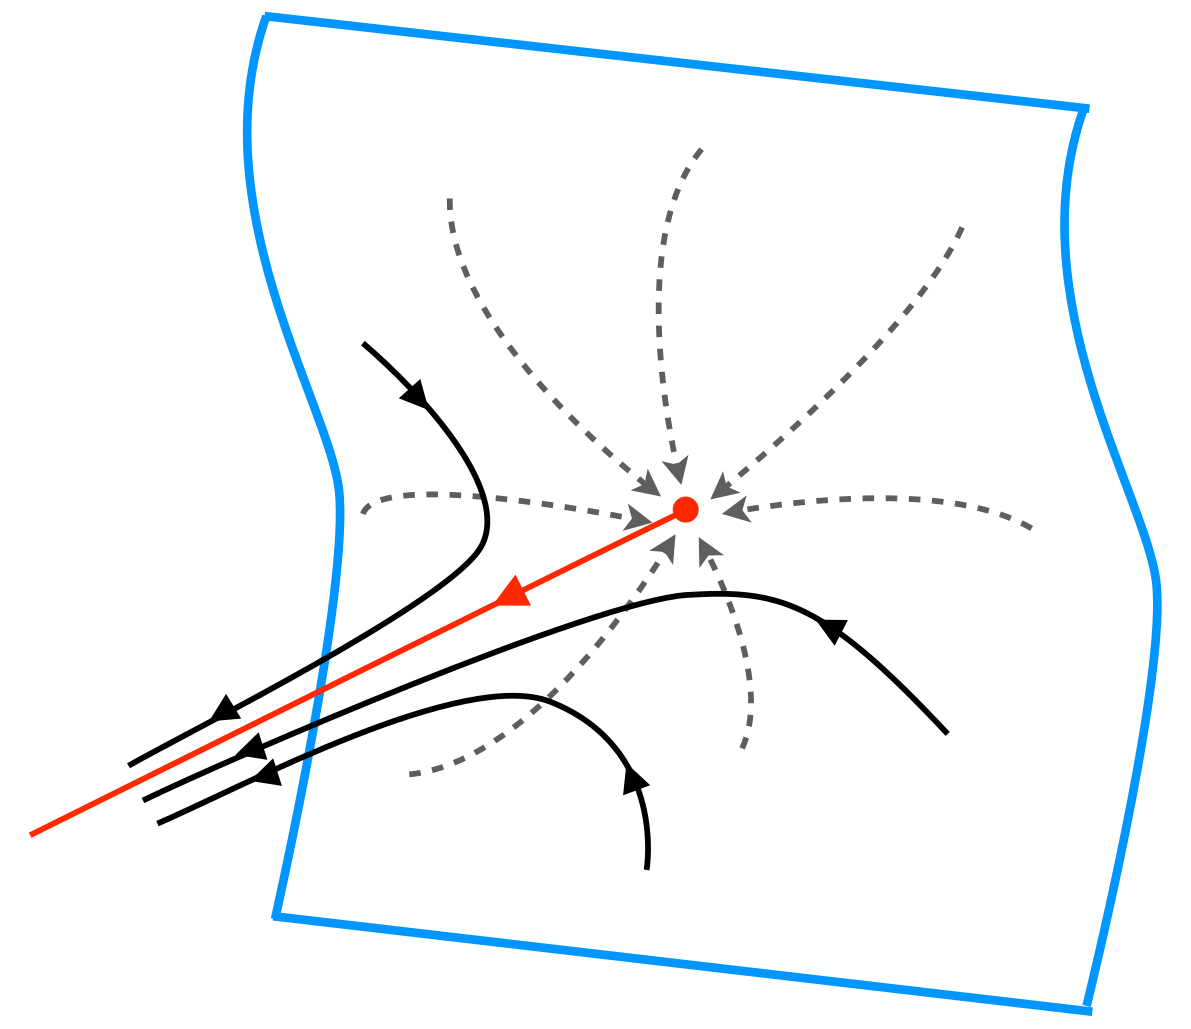
\includegraphics[width=.35\linewidth]{img/RG-flow.png}
	\end{figure}
\subsection{Physical Scales vs the Cutoff}
	LSZ reduction (with the ``mostly plus'' metric convention, see \textit{Srednicki}):
	\begin{equation}
		\int \dd[d]{x} e^{-ip\cdot x}
		\int \dd[d]{y} e^{+ik\cdot y}
		\ave[\big]{\phi(x)\,\phi(y)}
	\xmapsto{\ p,k\ \text{on-shell}\ }
		\frac{-i\sqrt{Z_\phi}}{p^2 + m^2 - i\epsilon}
		\frac{-i\sqrt{Z_\phi}}{k^2 + m^2 - i\epsilon}
		\mel{p}{S}{k}
	\end{equation}
	\begin{equation}
		\ave[\big]{\phi(x)\,\phi(y)}
		= \frac{1}{\mcal{Z}}
			\int \DD{\phi_\Lambda} e^{iS_\Lambda[\phi]}\,
			\phi(x)\,\phi(y)
	\end{equation}
	$S \sim \idty + i\mcal{M}(\mu)$, physical amplitude $\mcal{M}(\mu)$ scale with energy $\mu$, but is cutoff-independent. 
	
	How to relate $\mcal{M}(\mu)$ to $g(\Lambda)$? Note that the canonical Green function \textit{does} scale with $\Lambda$! With the help of Poincar\'e invariance, we have:
	\begin{equation}
		Z_\Lambda \ave[\big]{\phi(x)\,\phi(y)}
		\mathbin{=:} G_\Lambda\pqty\big{x,y; g(\Lambda)}
		= G_\Lambda\pqty\big{l; g(\Lambda)},
	\quad
		Z_\lambda := (Z_\phi)_\Lambda
	\end{equation}
	Physical scale: $l = \abs{x_1 - x_2}$, or center of mass momentum $\mu$ in amplitudes; $l\cdot \mu \sim 1$. $\Lambda$-dependence enters through $Z_\phi$. For general $n$-pt function, RG flow:
	\begin{equation}
	\begin{aligned}
		\ave[\big]{\phi^n(\cdots)}
		= \frac{1}{\mcal{Z}}
			\int \DD{\phi_\Lambda} e^{iS_\Lambda[\phi]}\,
			\phi^n(\cdots)
		&= Z^{-n/2}_\Lambda
			G_\Lambda \pqty\big{l; g(\Lambda)} \\
		&= Z^{-n/2}_{s\Lambda}
			G_{\Lambda} \pqty\big{sl; g(s\Lambda)}\,
			\pqty{s^{1 - \frac{d}{2}}}^{-n}
	\end{aligned}
	\end{equation}
	
	This is a key result! We have:
	\begin{equation}
		G_\Lambda \pqty\big{l; g(\Lambda)}
		= G_{\Lambda} \pqty\big{sl; g(s\Lambda)}
			\pqty{
				s^{1 - \frac{d}{2}}
				\sqrt{\frac{Z_\Lambda}{Z_{s\Lambda}}}
			}^n
		\simeq G_{\Lambda} \pqty\big{sl; g(s\Lambda)}
			\,s^{n\Delta_\phi}
	\end{equation}
	Or in terms of energy scale $\mu$,
	\begin{gather}
		\mcal{M} \pqty\big{\mu; g(\Lambda)}
		= \mcal{M} \pqty\big{\mu/s; g(s\Lambda)},
	\\[1ex]
		\mu\,\pdv{\mcal{M}}{\mu}
		= \pdv{M}{g}\,\pqty{
				\Lambda\,\pdv{g}{\Lambda}
			}
	\end{gather}
\section{Perturbative Renormalization}
	However, in naïve perturbation theory, we wish to complete the entire
	path integral $\mcal{Z} (g_0,\Lambda_0)$. We can think of this as
	integrating out more and more high energy modes, until we reach the IR
	scale $\Lambda \to 0$.
	
	When $\Lambda \ll \Lambda_0$, we have no reason to believe the
	renormalized couplings $g(\Lambda)$ are close to the original
	couplings $g_0$ at $\Lambda_0$. In fact, they may differ by a large
	(but finite) renormalization factor $Z$: $g_0 = Zg$.
	
\subsection{Counterterms}
	In the above analysis, the theory flows from UV to IR. However, in
	reality, the IR results are known from experiments, and we are trying to
	\emph{extrapolates} from IR to UV.
	
	We achieve this by \emph{tuning} the bare parameters $(g_0,\Lambda_0)$
	so that after RG flow, the IR results fit our experimental observations.
	If the IR couplings $g(\Lambda)$ are finite and small, then since
	$\Lambda \ll \Lambda_0$, we expect $g_0$ to be very large.
	
	We often \emph{split} $g_0$ into 2 parts for convenience:
	\begin{equation}
	  g_0 = g + \var{g}
	  = g + (Z - 1)\,g
	\end{equation}
	$\var{g}$ is the so-called \emph{counterterm}; intuitively, it's the
	(large) correction that gets integrated out when we go from
	$\Lambda_0$ all the way to IR.
	
	Basically, we have the following procedure:
	
	\begin{figure}[!h]
	\centering
	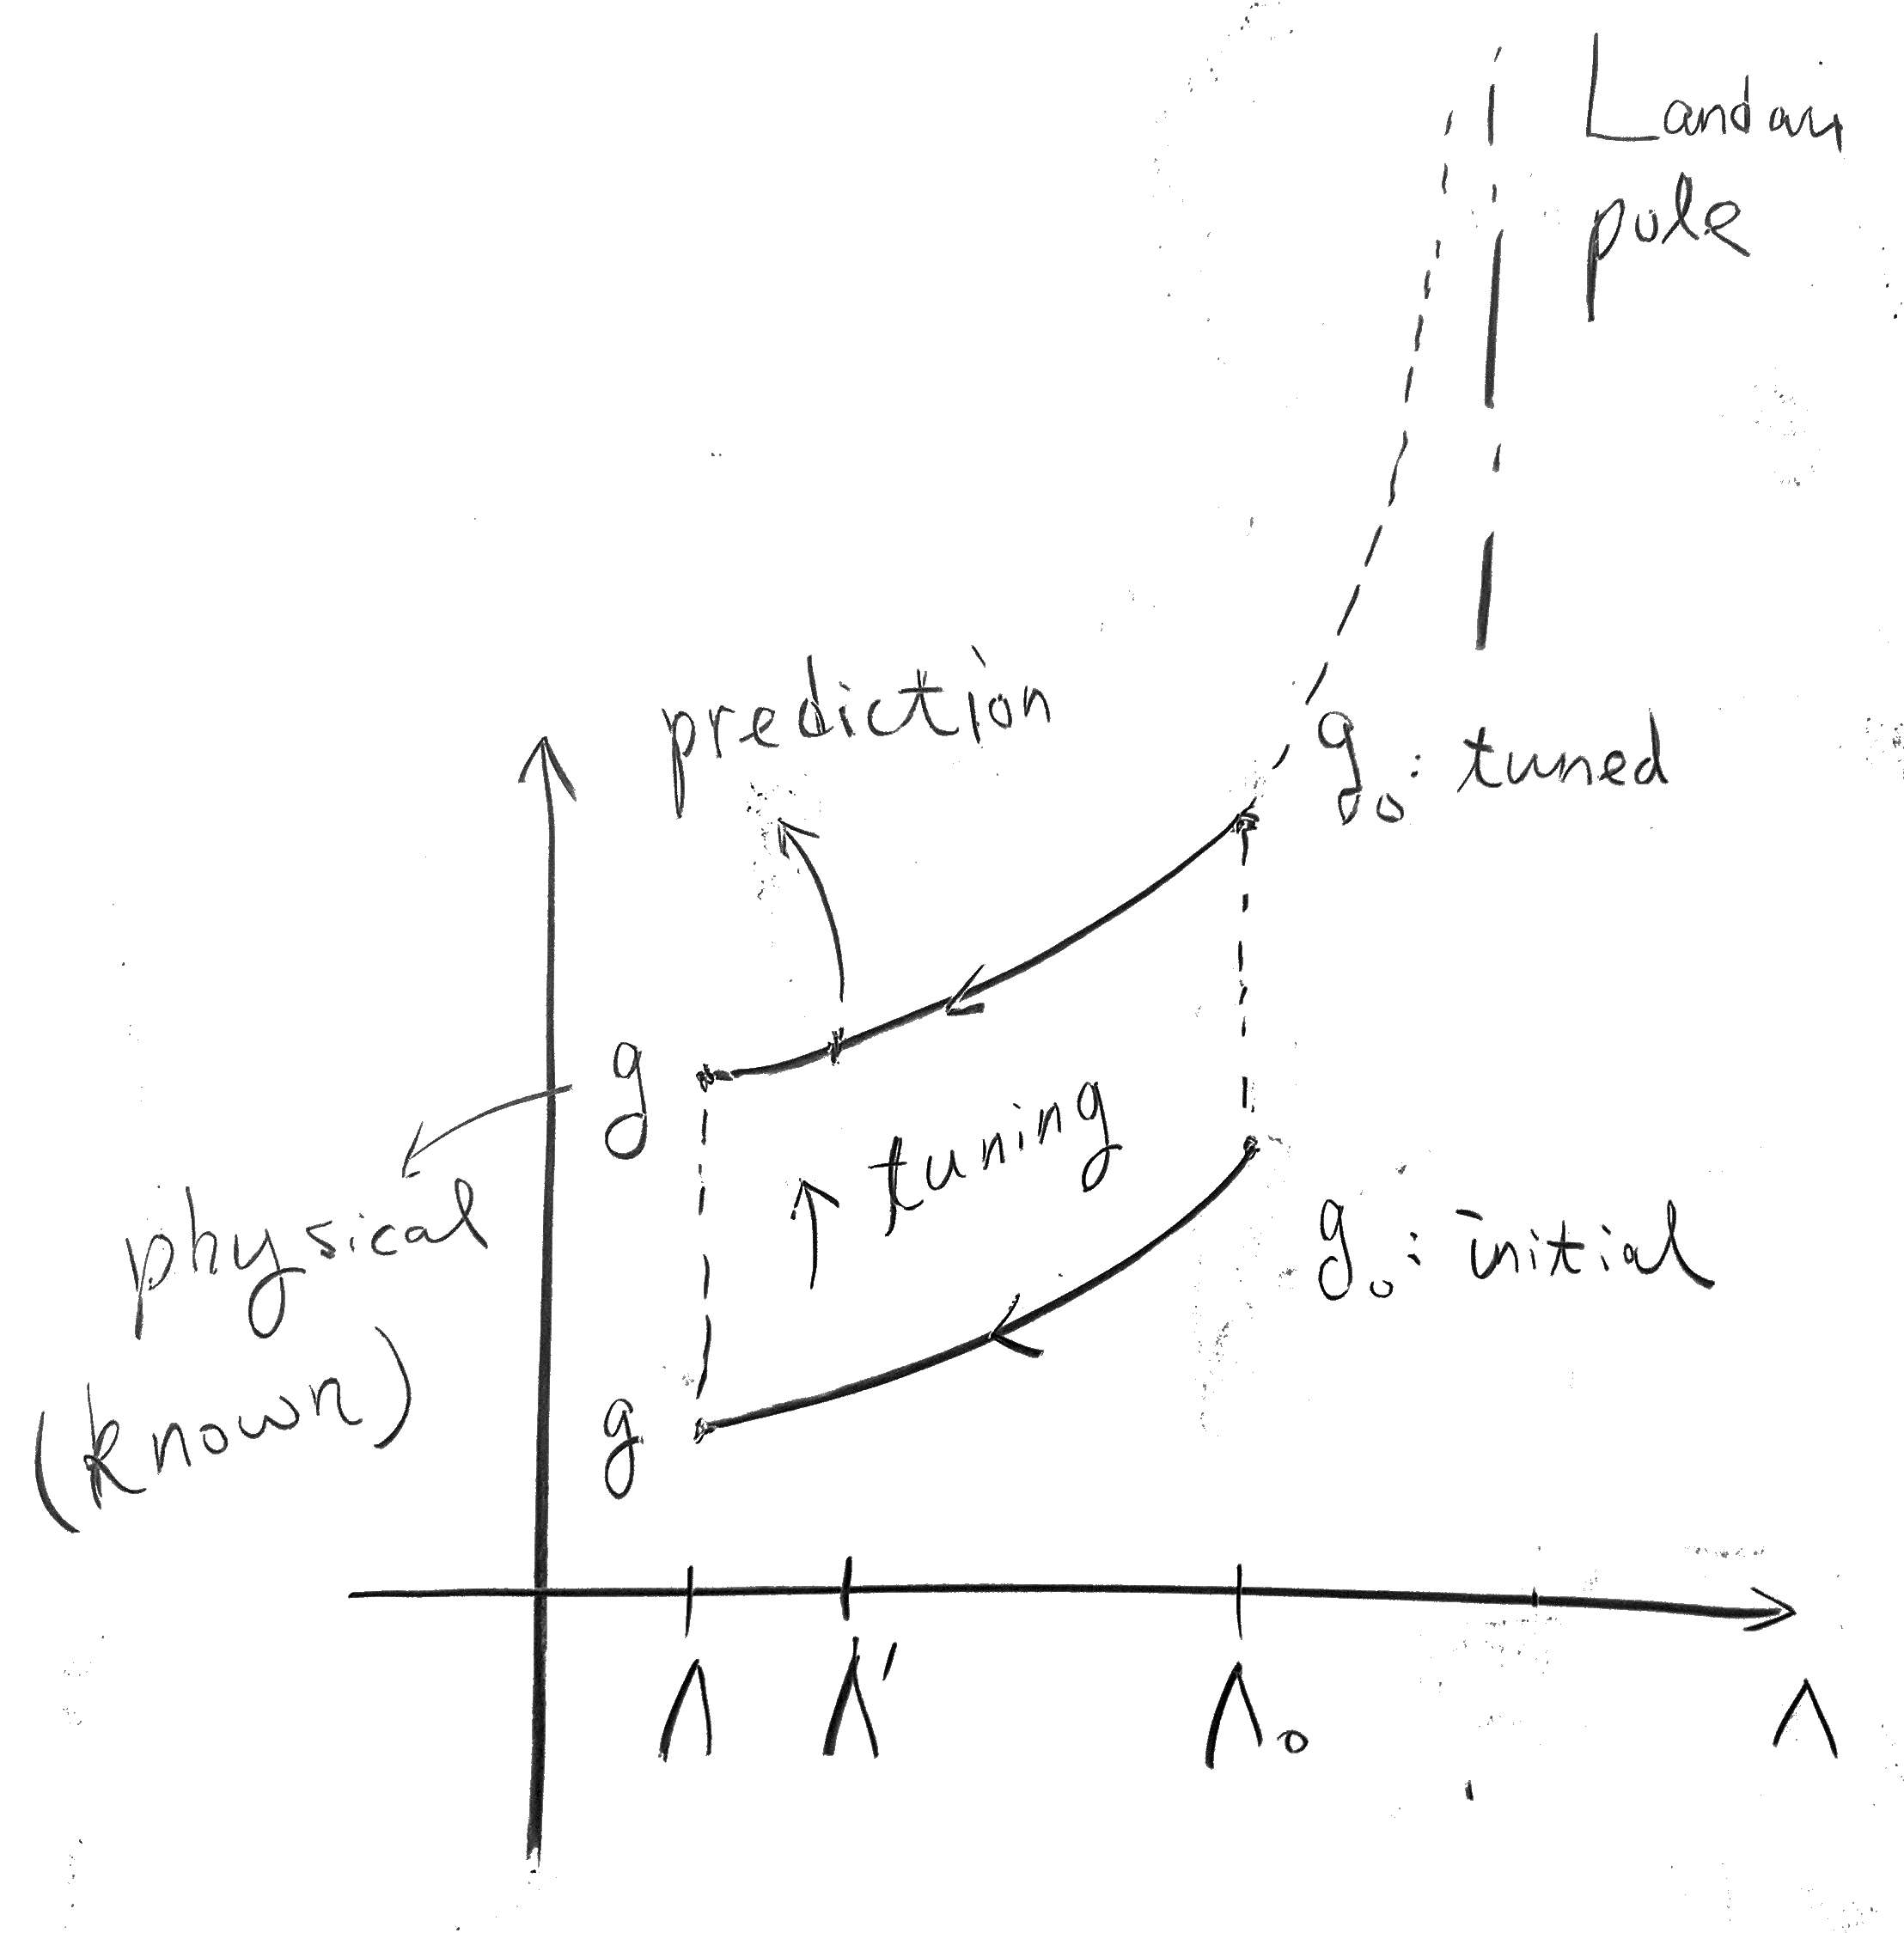
\includegraphics[width=.5\linewidth]{img/RG-process.png}
	\end{figure}
	
	\begin{enumerate}[noitemsep,midpenalty=100]
	\setcounter{enumi}{-1}
	
	\item
	  Select some UV parameters $(g_0,\Lambda_0)$
	\item
	  Perform the RG flow: $(g_0,\Lambda_0)\to (g,\Lambda)$
	\item
	  Tune (redefine) $g_0$ so that $(g,\Lambda)$ matches with
	  experiments
	\item
	  Use the tuned data to predicts phenomena at a different scale
	  $(g',\Lambda')$
	\end{enumerate}
	
	Note that the tuning of UV parameters $g_0$ is \emph{far from unique!}
	This is easy to understand: many UV theories might flow to the same IR
	theory. For this reason, some would say that RG is a \emph{semi-group}.
	
	However, for a \emph{renormalizable} theory, we can restrict the tuning
	to a \emph{finite} dimensional subspace formed by the \emph{relevant}
	couplings, since most other parameters $g^{(i)}$ are \emph{irrelevant}
	and get suppressed by $\Lambda/\Lambda_0$ in the IR. We shall see this in more details later. After such
	restriction to a relevant subspace, the RG flow is a group, and we can
	reverse the flow to \emph{extrapolate} towards UV.
	
	\begin{quote}
	\textbf{Subtlety:} the tuning process described above might encounter some serious
	obstruction: the tuned $g_0$ could blow up at some finite
	$\Lambda_{\mathrm{UV}}$; this is the so-called \emph{Landau pole}.
	This tells us that the theory only works under some
	$\Lambda_{\mathrm{UV}}$, i.e.~it is not \emph{UV complete}; it's only
	an \emph{effective} theory. One have to ``embed'' this Lagrangian into a
	bigger theory that works beyond $\Lambda_{\mathrm{UV}}$; this is the
	non-trivial \emph{UV completion} of an effective theory.
	\end{quote}
	
\subsection{Perturbation}
	The above results are non-perturbative and should always hold.
	Perturbation theory is only a way to calculate the RG flow from UV to
	IR; it is reliable only if the IR coupling $g$ is sufficiently small.
	In this case we can tune $(g_0,\Lambda_0)$ with the following
	recursive / iterative algorithm:
	
	\begin{enumerate}[noitemsep]
	\item
	  Perturbative calculation of RG flow:
	  $(g_0,\Lambda_0)\to (g,\Lambda)$ at $\order{g^n}$
	\item
	  Tune (redefine) $(g_0,\Lambda_0)$ by adding counterterms, so that
	  $(g,\Lambda)$ matches with experiments
	\item
	  Increase order $n$ and go to step 1
	\end{enumerate}
	
	The (non-)renormalizability of a theory is evident in the perturbative
	expansion, by counting the \textbf{superficial degrees of divergence}
	$D$ of the Feynman diagrams. Basically,
	
	\begin{itemize}
	\item
	  Interaction vertices create loops, and loops create UV divergences.
	  Higher order interaction vertices create more loops, which lead to
	  more divergences.
	\item
	  External lines suppress UV divergences by factors like
	  $\frac{1}{\cancel{p}}$ or $\frac{1}{p^2}$.
	\end{itemize}
	
	For a renormalizable theory, there will be no divergence for diagrams
	with a sufficient number $E$ of external legs; for a
	non-renormalizable theory, however, there will always be divergences, no
	matter how large $E$ is.
	
\subsection{Renormalization Schemes}
	
	There is a subtlety in the above procedure: how do we actually relate IR
	parameters $(g,\Lambda)$ with actual physical quantities,
	e.g.~amplitudes $\mcal{M}(\mu)$?
	
	In fact, we've assumed that $(g,\Lambda)_{\Lambda\to 0}$ gives the
	physical couplings that we are familiar with, e.g.~mass, electric charge
	and so on. This is not quite true, since physical quantities are
	actually defined with scattering amplitudes. There are different choices
	of relating $g$ with physical observables; this lead to various
	renormalization schemes:
	
	\begin{itemize}[nosep]
	
	\item
	  On-shell / pole-mass scheme
	\item
	  Minimal subtraction ($\mathrm{MS}$) \& modified MS
	  ($\overline{\mathrm{MS}}$)
	\end{itemize}
	
\section{Renormalizability}
	As we've mentioned before, most parameters $g^{(i)} \in g$ are, in fact, \emph{irrelevant} --- such terms in the Lagrangian get suppressed by $\Lambda/\Lambda_0$ in IR. We shall see how this arise from dimensional anlaysis.
	
	
	
	If the IR theory has only \emph{relevant} couplings, then one should be
	able to recover their physical values by tuning a finite amount of
	relevant couplings in the UV, and usually the tuning is unique. This is
	the defining characteristic of a \textbf{renormalizable} theory.
	Basically, this means that we can naturally obtain a UV theory by
	extrapolation.
	
	On the other hand, a theory is \textbf{non-renormalizable} if it
	contains irrelevant couplings in the IR. In this case the IR parameters
	$g$ depend sensitively on small perturbations of the UV parameters
	$g_0$, and one has to tune infinitely many bare parameters to obtain
	the physical IR values. Such theory is hardly \emph{fundamental}, since
	it depends on infinitely many parameters; but it's a good
	\emph{effective theory} nonetheless.
	
\section{Effective Action}
	After $\phi_\Lambda$ is completely integrated out, we
	have:
	
	\begin{equation}
	  S_{\mathrm{eff}}[\phi] \to W,\quad
	  Z(g_0,\Lambda_0) = e^{iW}
	\end{equation}
	Note that $W$ no longer has any $\phi$ dependence, but it is a
	function of $(g_0,\Lambda_0)$, which in turn is tuned by physical
	$(g,\Lambda)$. $W$ in fact contains all information about the seed
	theory, labeled by $(g_0,\Lambda_0)$. To extract this information, we
	usually perturb the original action $S[\phi]$ with a source term; then
	we have:
	
	\begin{equation}
	  S[\phi,J]
	  = S[\phi] + \int \dd{x}\,J(x)\,\phi(x),\quad
	  W \to W[J]
	\end{equation}
	
	Expand $W[J]$ in terms of $J$-modes, and its coefficient gives us
	physical coupling constants in the IR. More precisely, we can define the Legendre-transformed $\Gamma[\varphi]$.


\printbibliography[%
%	title = {参考文献} %
	,heading = bibintoc
]
\end{document}
